%%%%%%%%%%%%%%%%%%%%%%%%%%%%%%%%%%%%%%%%%%%%%%%%%%%%%%%%%%%%%%%%%%%%%%%%%%%
%
% Generic template for TFC/TFM/TFG/Tesis
%
% $Id$
%
% By:
%  + Javier Mac�as-Guarasa.
%    Departamento de Electr�nica
%    Universidad de Alcal�
%  + Roberto Barra-Chicote.
%    Departamento de Ingenier�a Electr�nica
%    Universidad Polit�cnica de Madrid
%
% Based on original sources by Roberto Barra, Manuel Oca�a, Jes�s Nuevo,
% Pedro Revenga, Fernando Herr�nz and Noelia Hern�ndez. Thanks a lot to
% all of them, and to the many anonymous contributors found (thanks to
% google) that provided help in setting all this up.
%
% See also the additionalContributors.txt file to check the name of
% additional contributors to this work.
%
% If you think you can add pieces of relevant/useful examples,
% improvements, please contact us at (macias@depeca.uah.es)
%
% Copyleft 2013
%
%%%%%%%%%%%%%%%%%%%%%%%%%%%%%%%%%%%%%%%%%%%%%%%%%%%%%%%%%%%%%%%%%%%%%%%%%%%

\chapter{Desarrollo hardware}
\label{cha_desarrollo_hardware}

\begin{FraseCelebre}
  \begin{Frase}
No entiendes realmente algo a menos que seas capaz de explic�rselo a tu abuela.    
  \end{Frase}
  \begin{Fuente}
Albert Einstein
  \end{Fuente}
\end{FraseCelebre}


\section{Arquitectura hardware}

\begin{figure}[H]
\centering
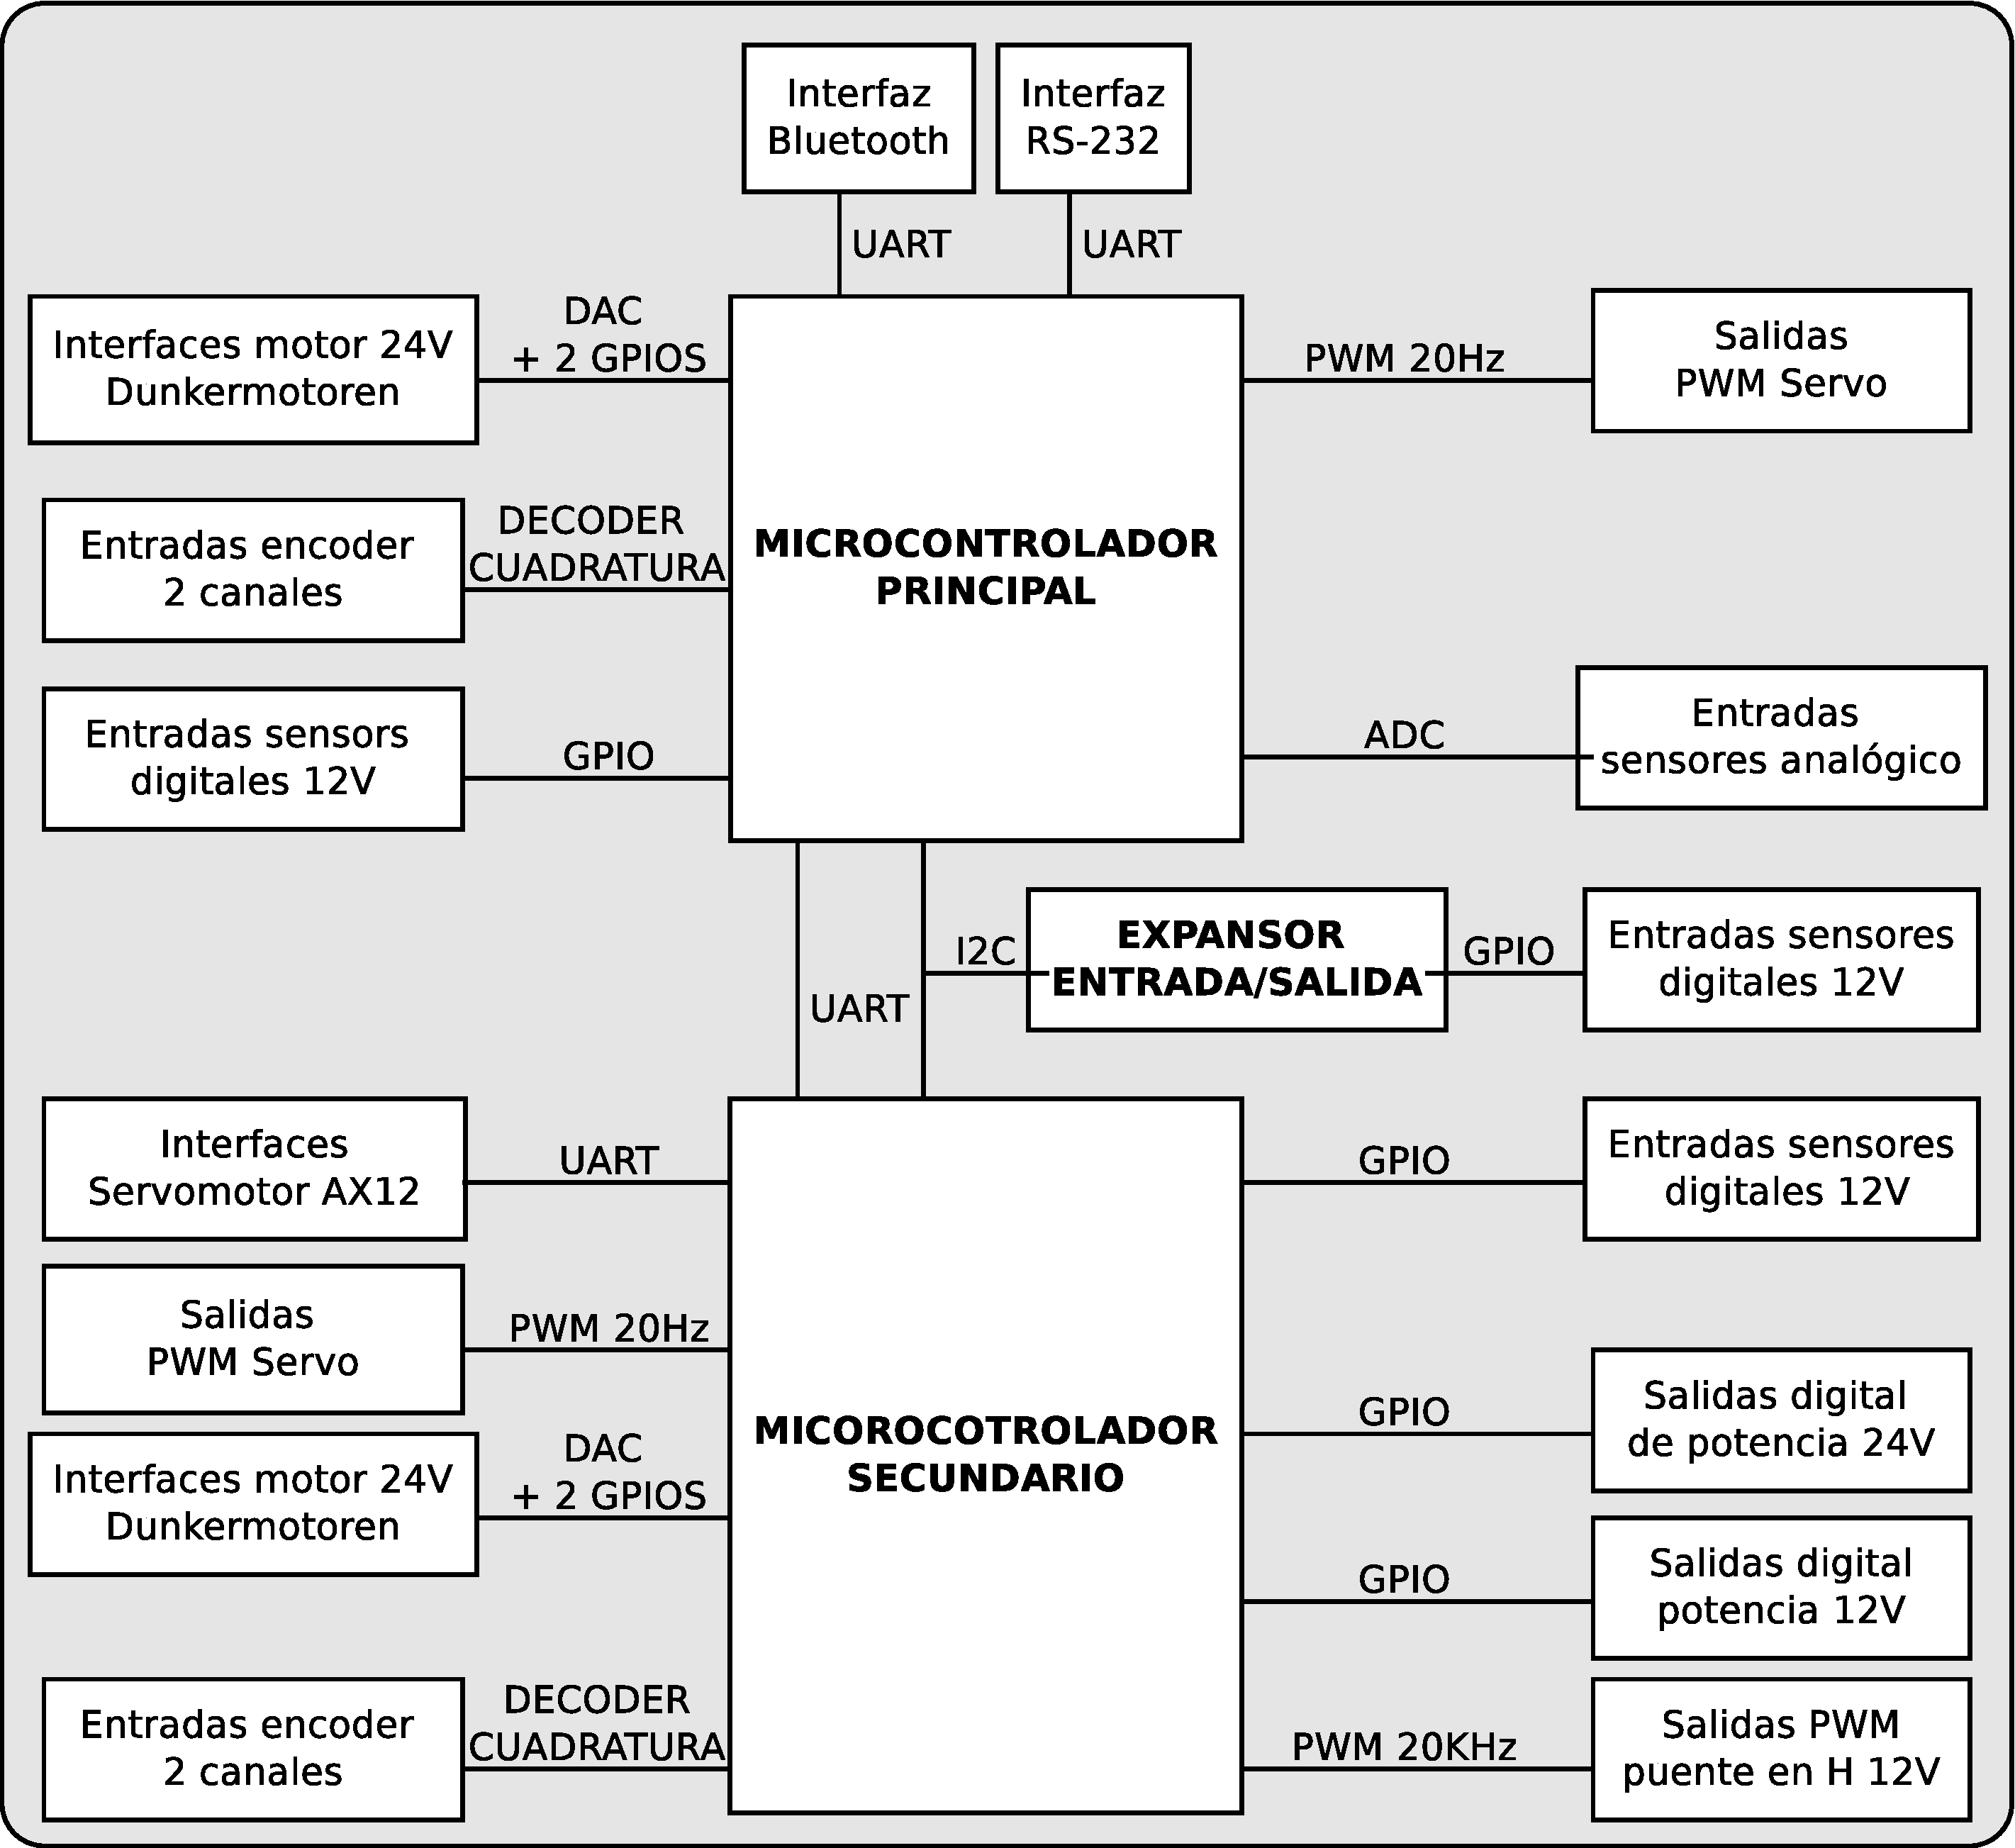
\includegraphics[width=.9\textwidth]{hardware_arquitectura_principal}
\caption[]{Arquitectura hardware principal}
\label{fig_hardware_arquitectura_principal}
\end{figure}

\subsection{Plataforma rob�tica base}

\begin{figure}[H]
\centering
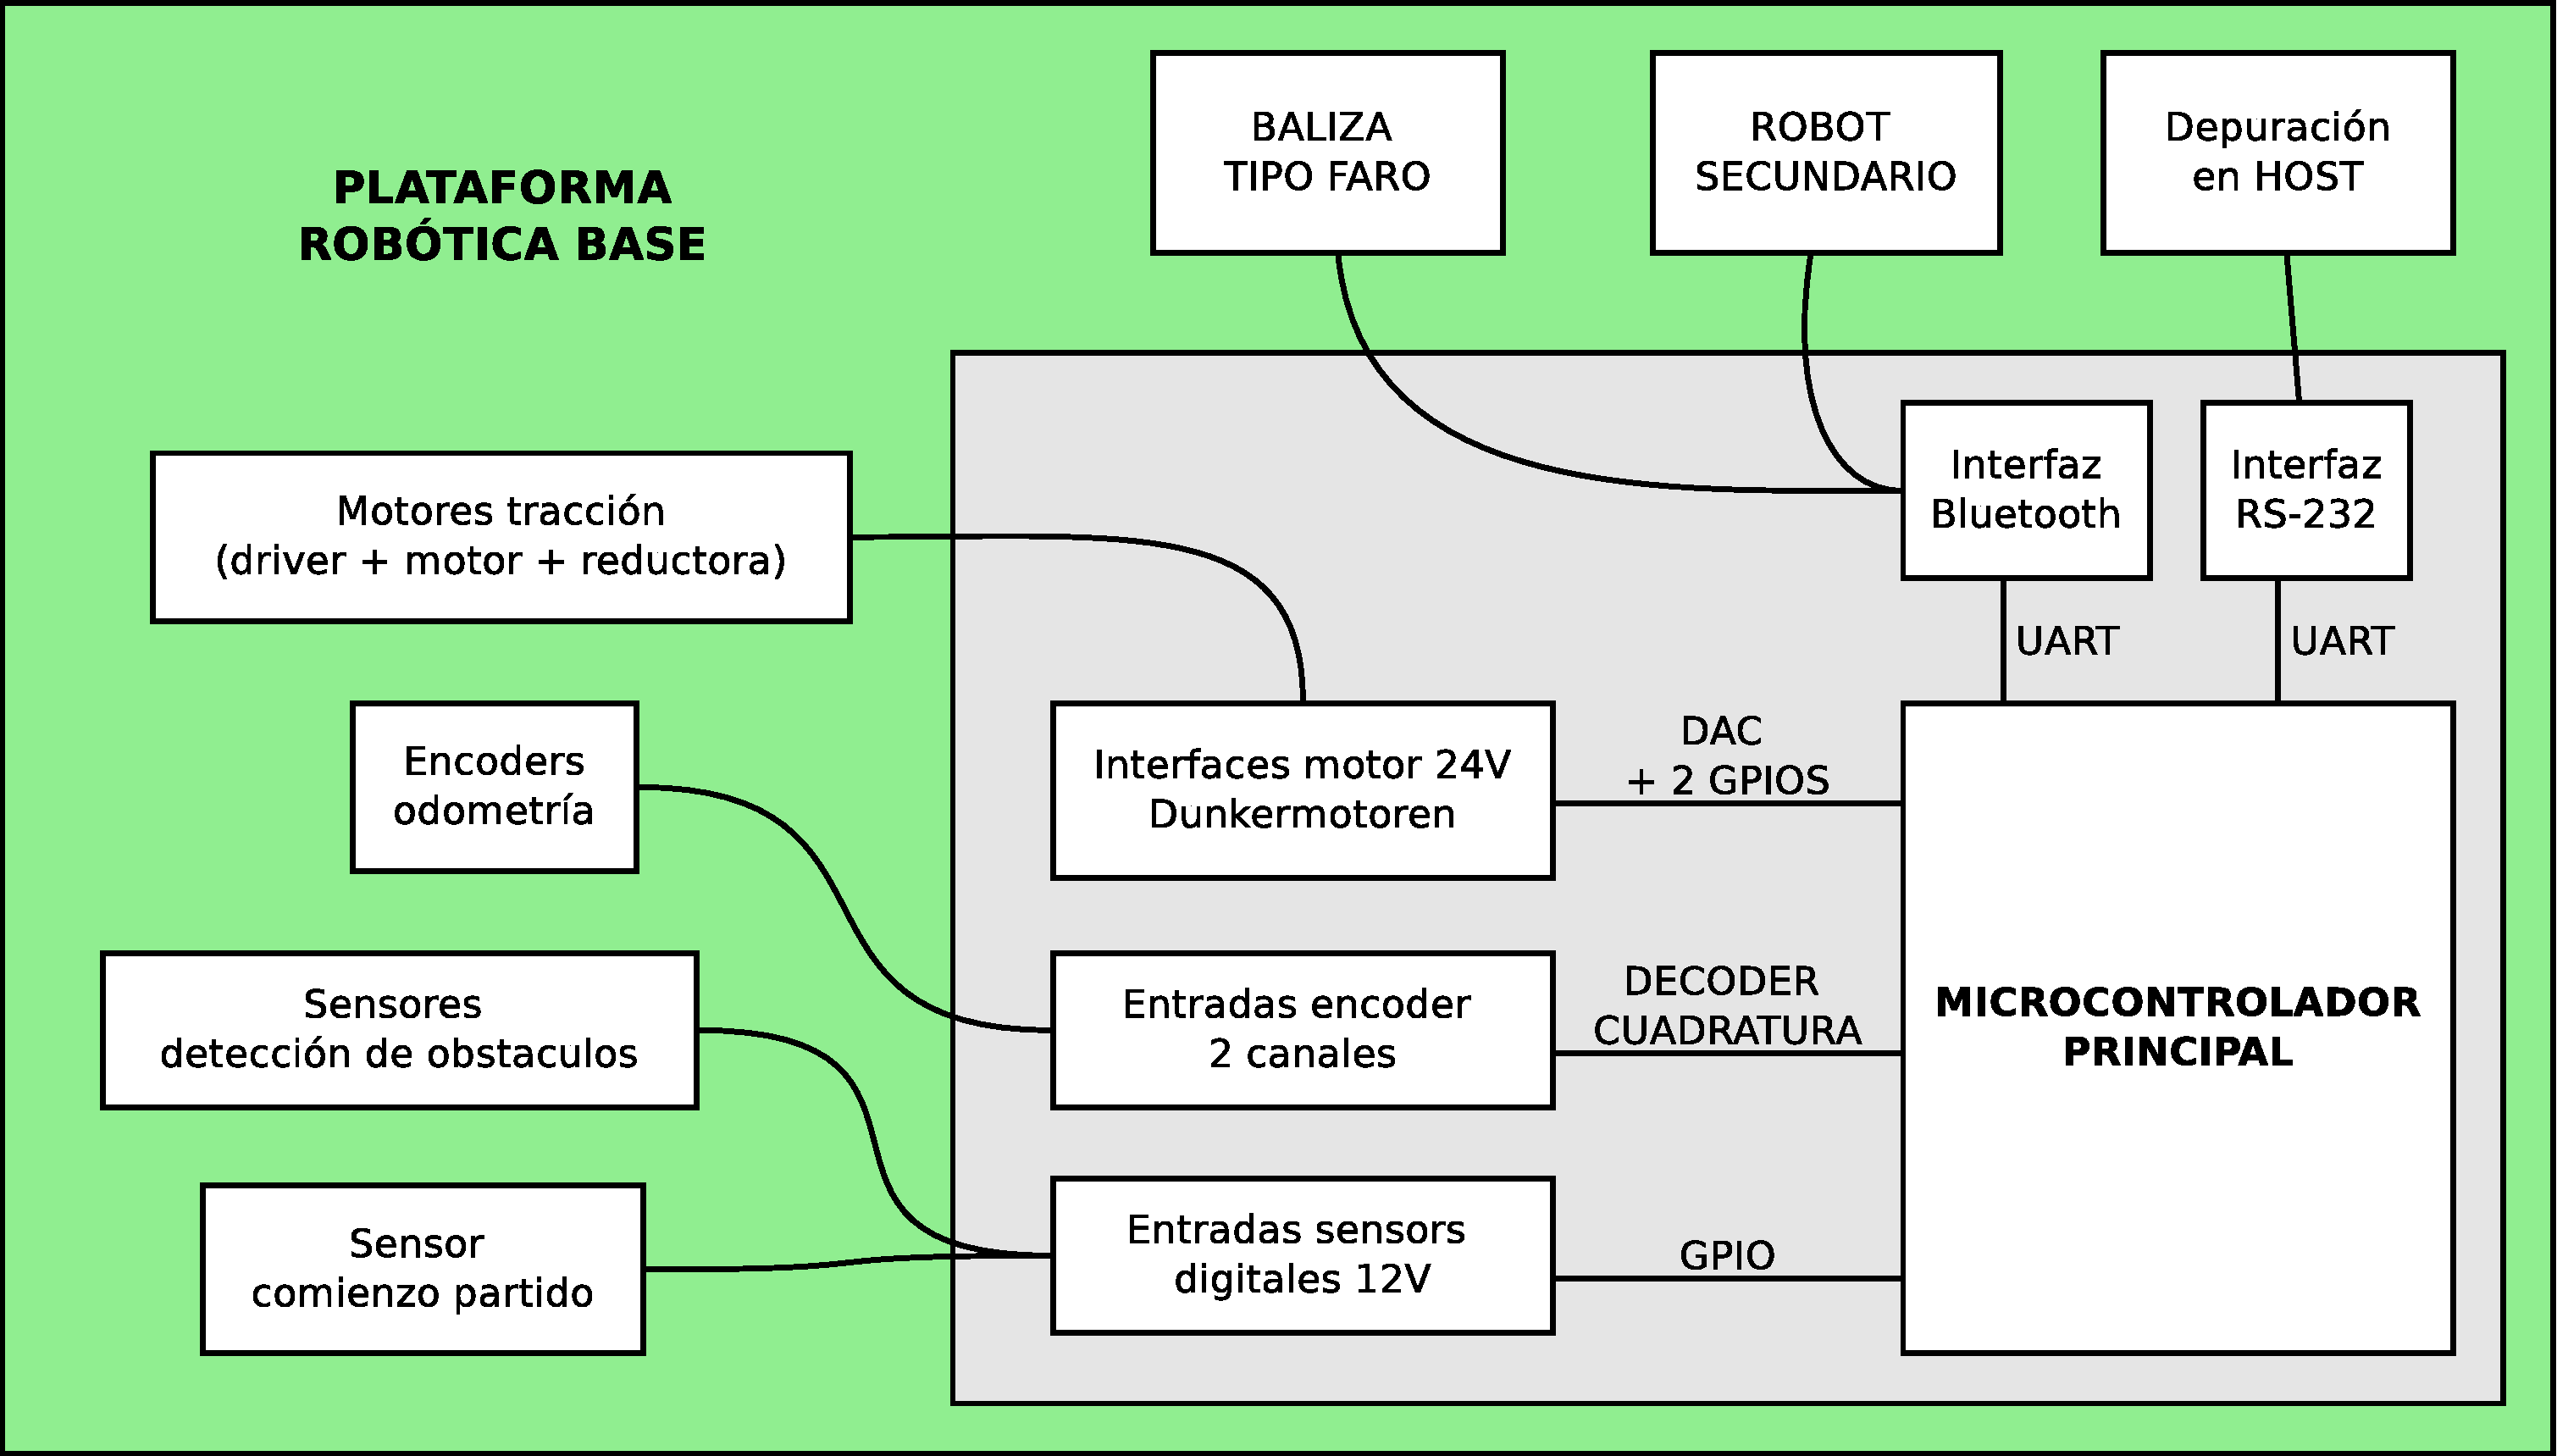
\includegraphics[width=.9\textwidth]{hardware_arquitectura_platafoma_robotica}
\caption[]{Recursos de hardware destinados a la plataforma rob�tica base}
\label{fig_hardware_arquitectura_plataforma_robotica}
\end{figure}

\subsection{Sistemas mec�nicos}

\begin{figure}[H]
\centering
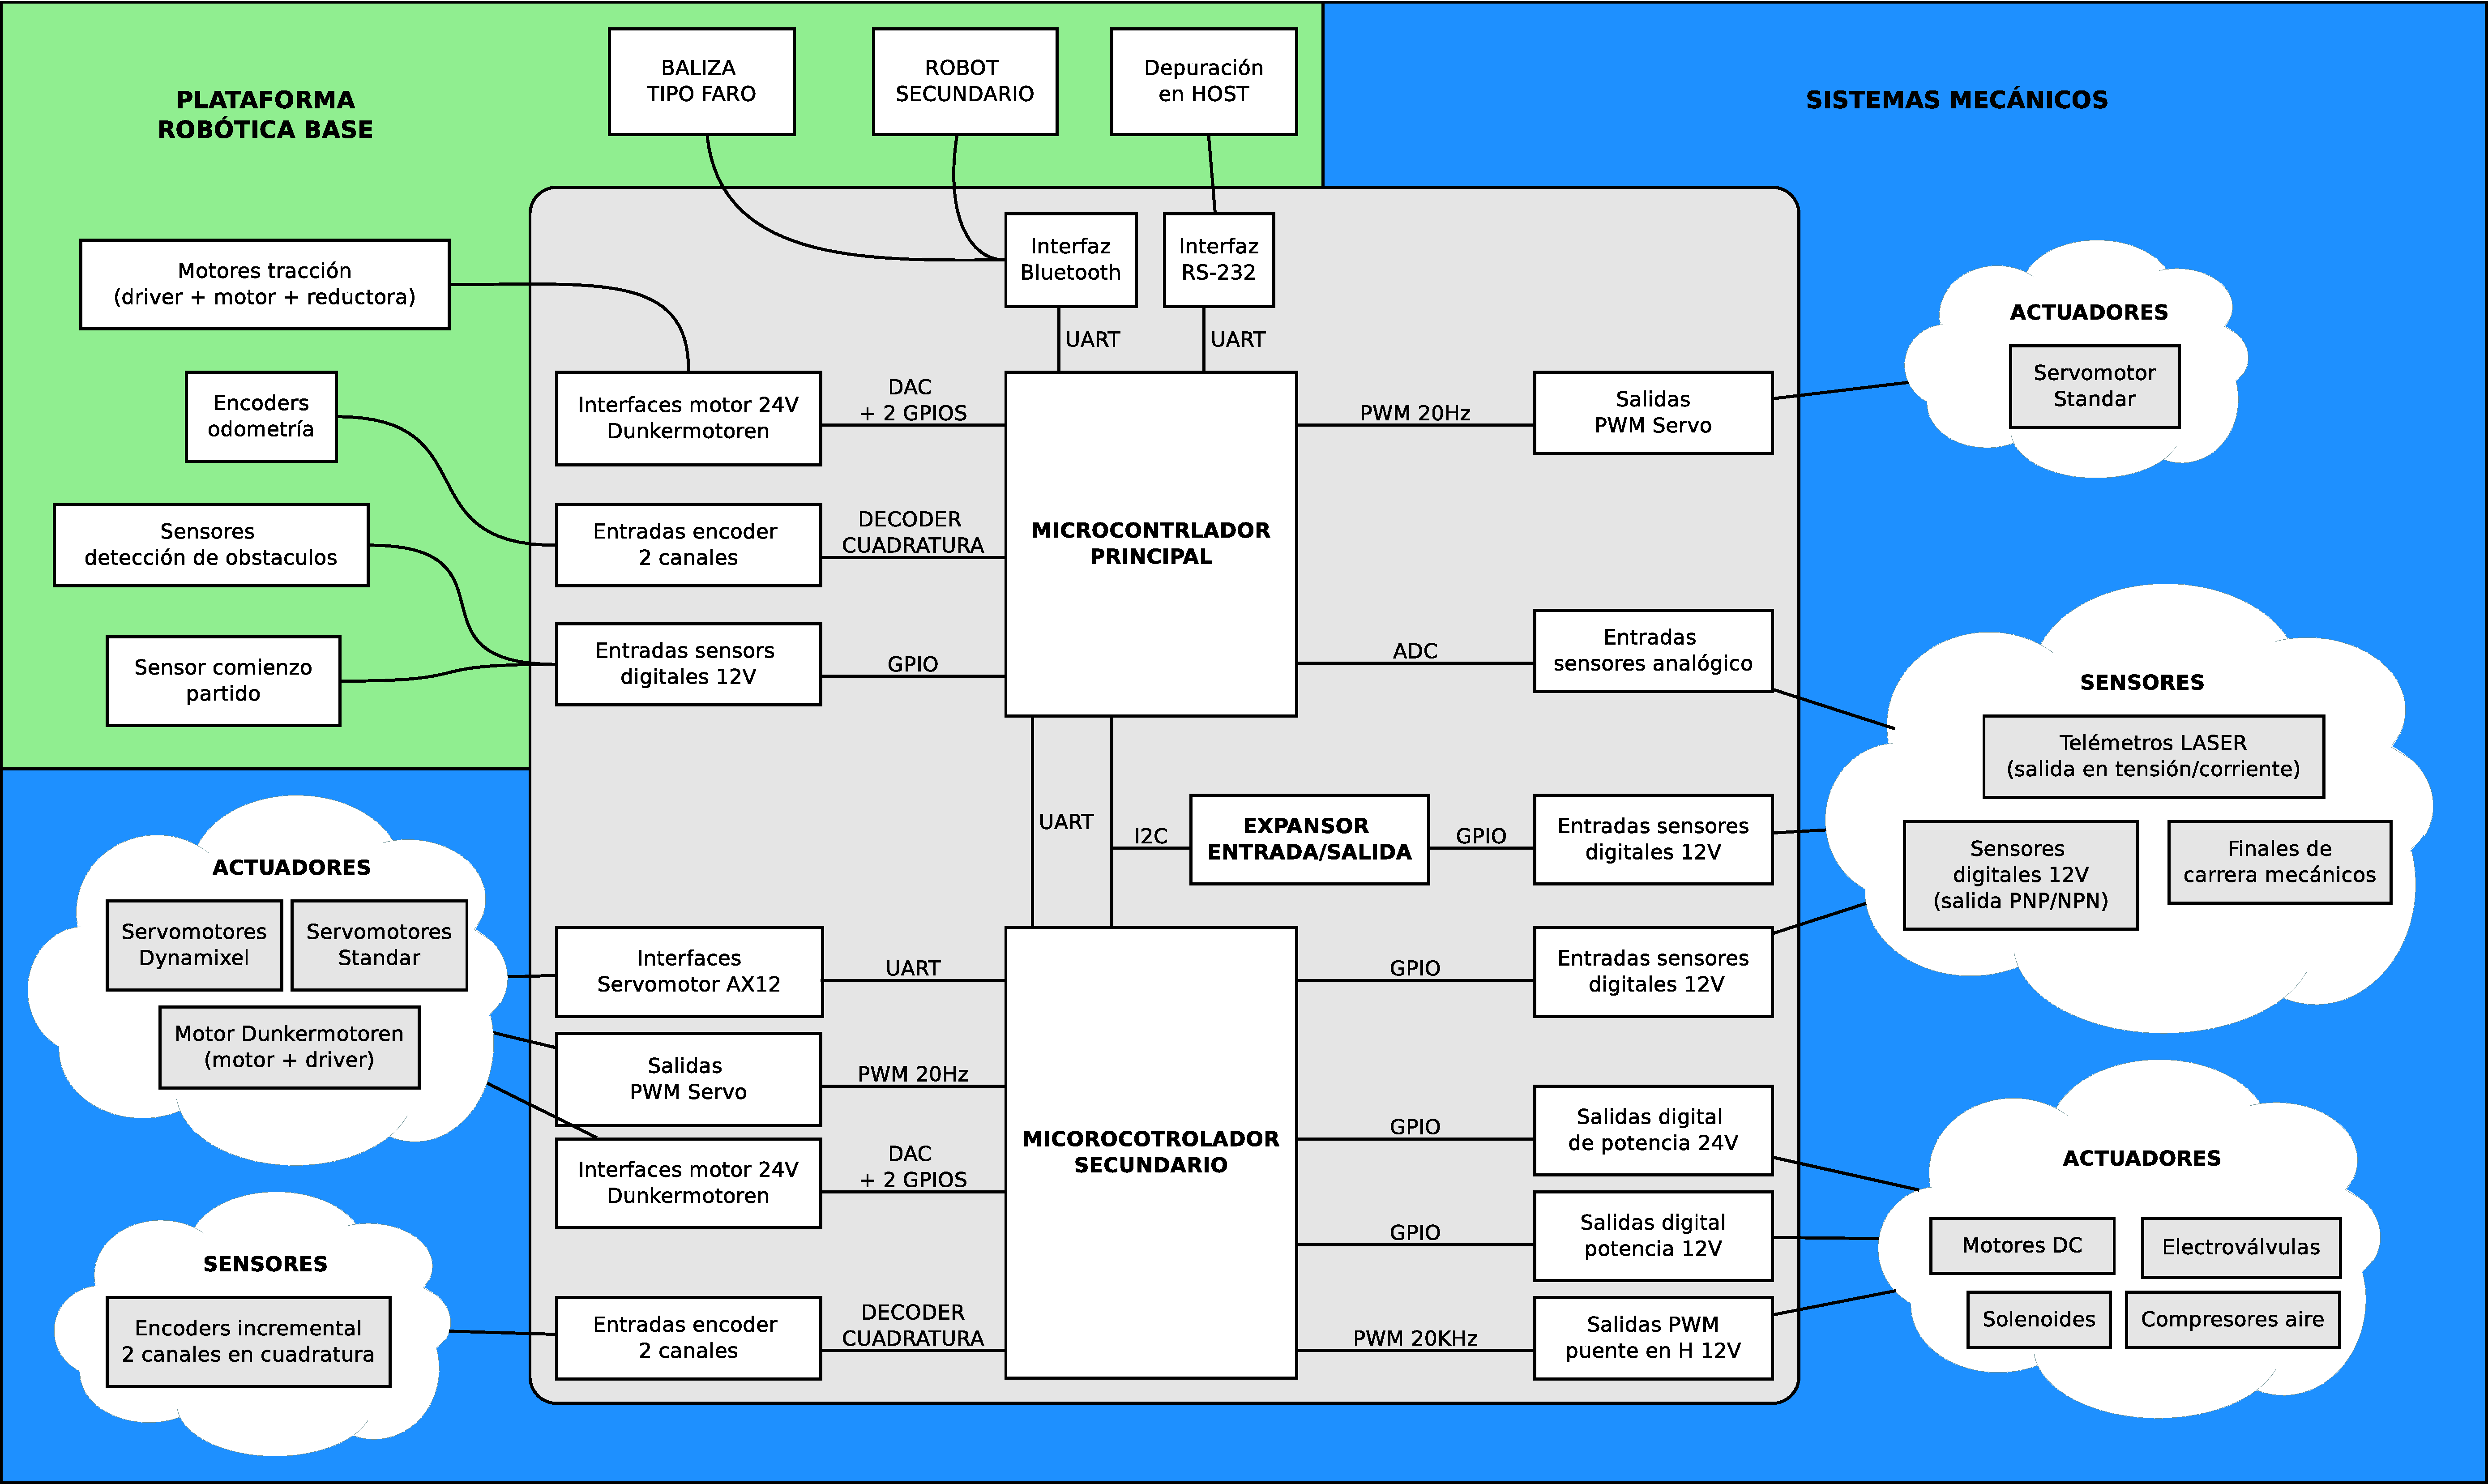
\includegraphics[height=.9\textwidth, angle=90]{hardware_arquitectura}
\caption[]{Recursos hardware destinados a la plataforma rob�tica y a los sistemas mec�nicos}
\label{fig_hardware_arquitectura}
\end{figure}

\subsection{�rbol de alimentaci�n}

\begin{figure}[H]
\centering
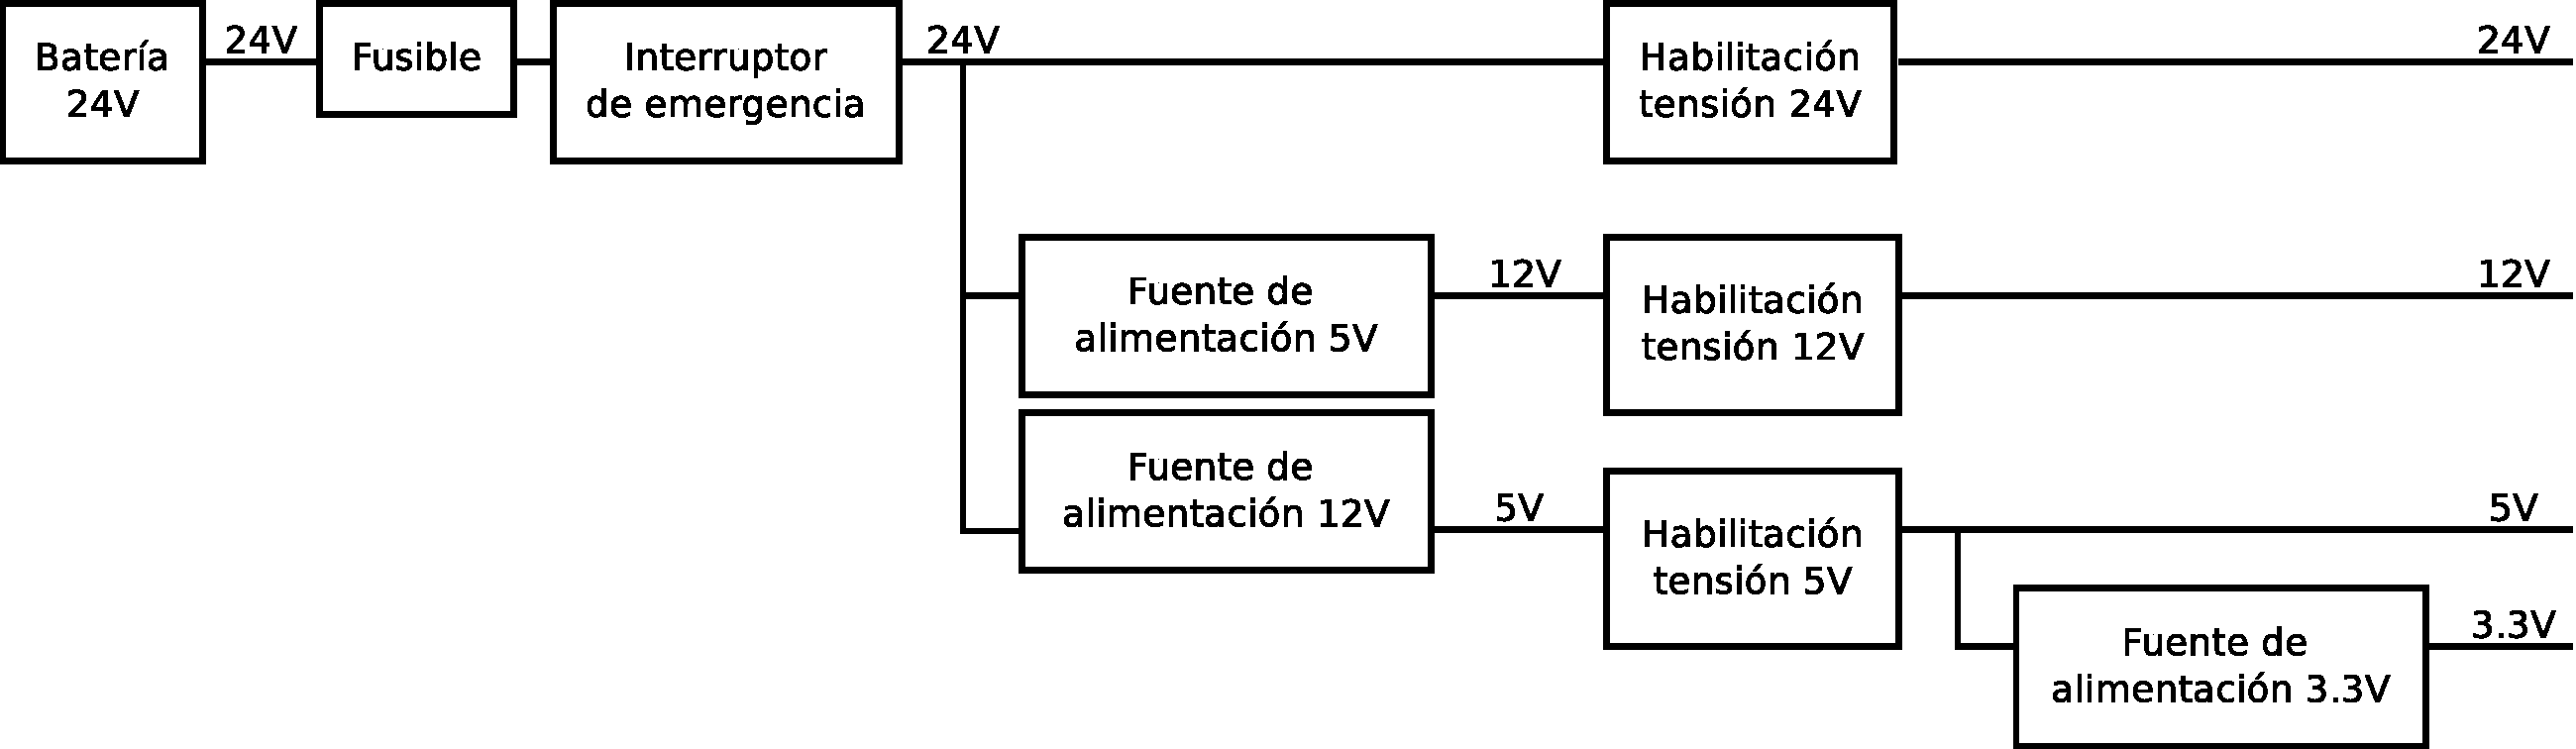
\includegraphics[width=.9\textwidth]{hardware_arquitectura_alimentacion}
\caption[]{Arquitectura hardware del �rbol de alimentaci�n del robot de Eurobot}
\label{fig_hardware_arquitectura_alimentacion}
\end{figure}

\section{Implementaci�n HW del robot principal}

\begin{figure}[H]
\centering
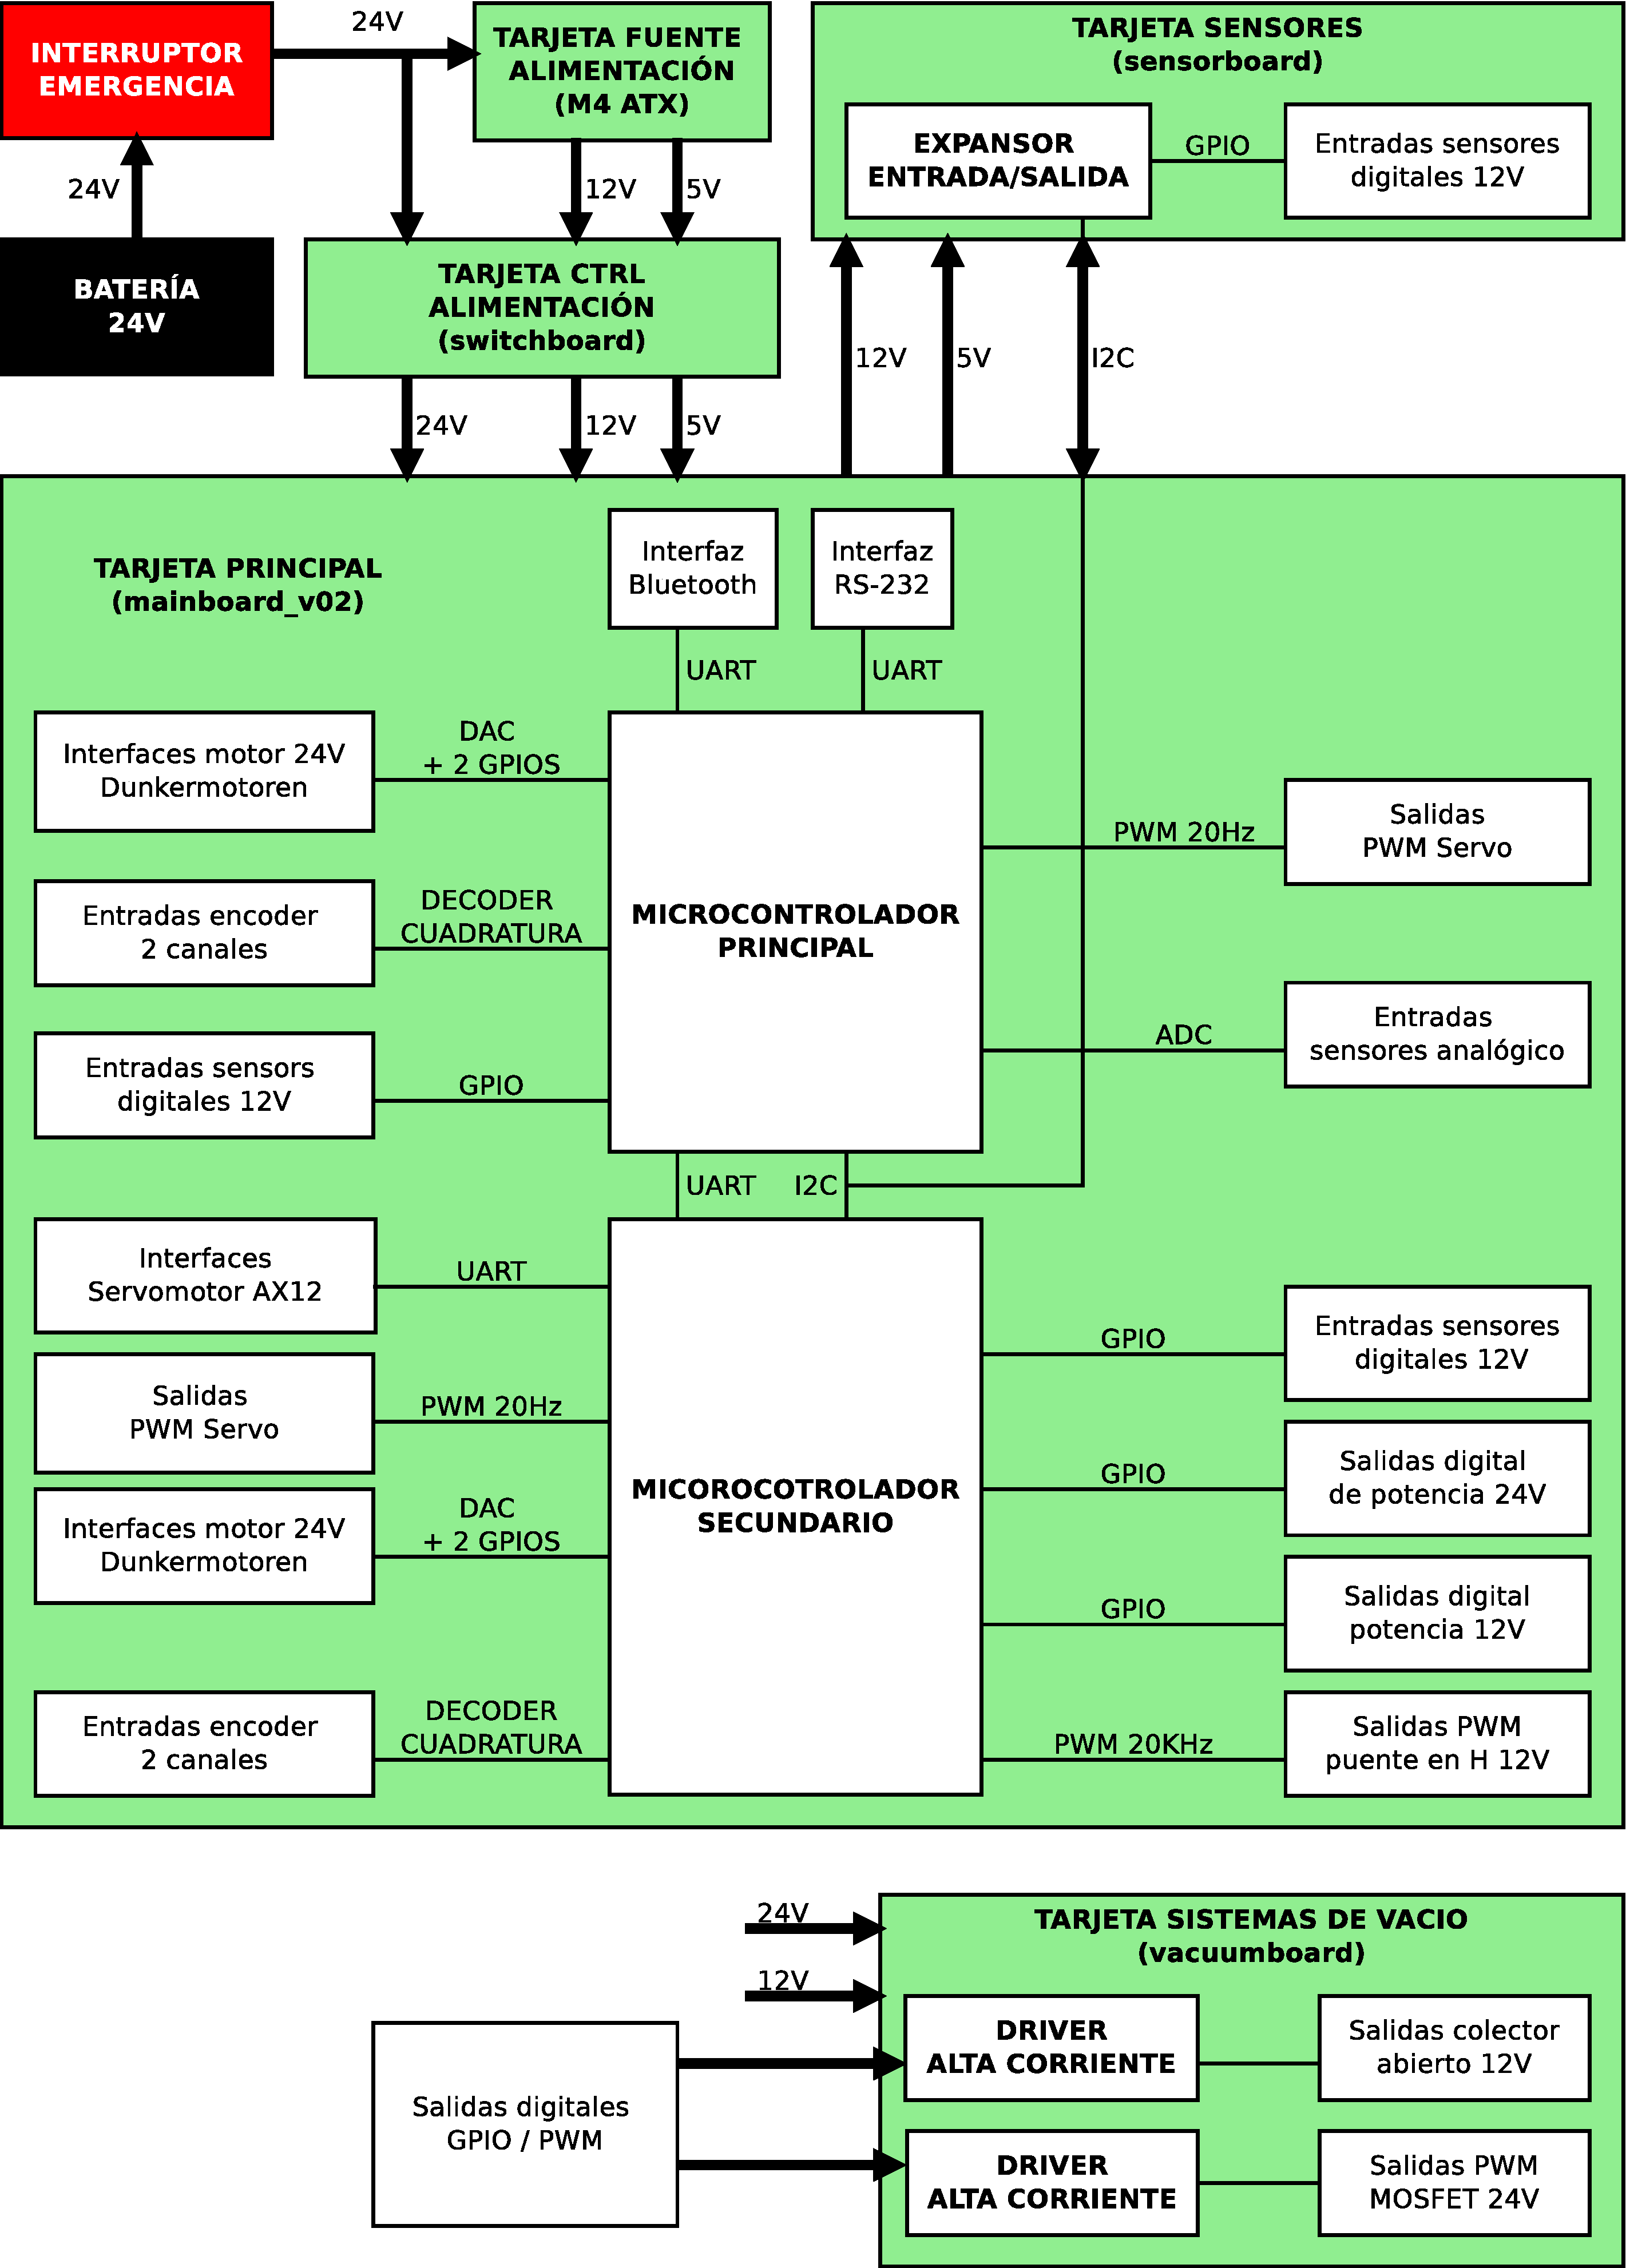
\includegraphics[width=.9\textwidth]{hardware_robot_principal}
\caption[]{Diagrama de bloques del HW del robot principal}
\label{fig_hardware_robot_principal}
\end{figure}


\subsection{Tarjeta principal}

\begin{figure}[H]
\centering
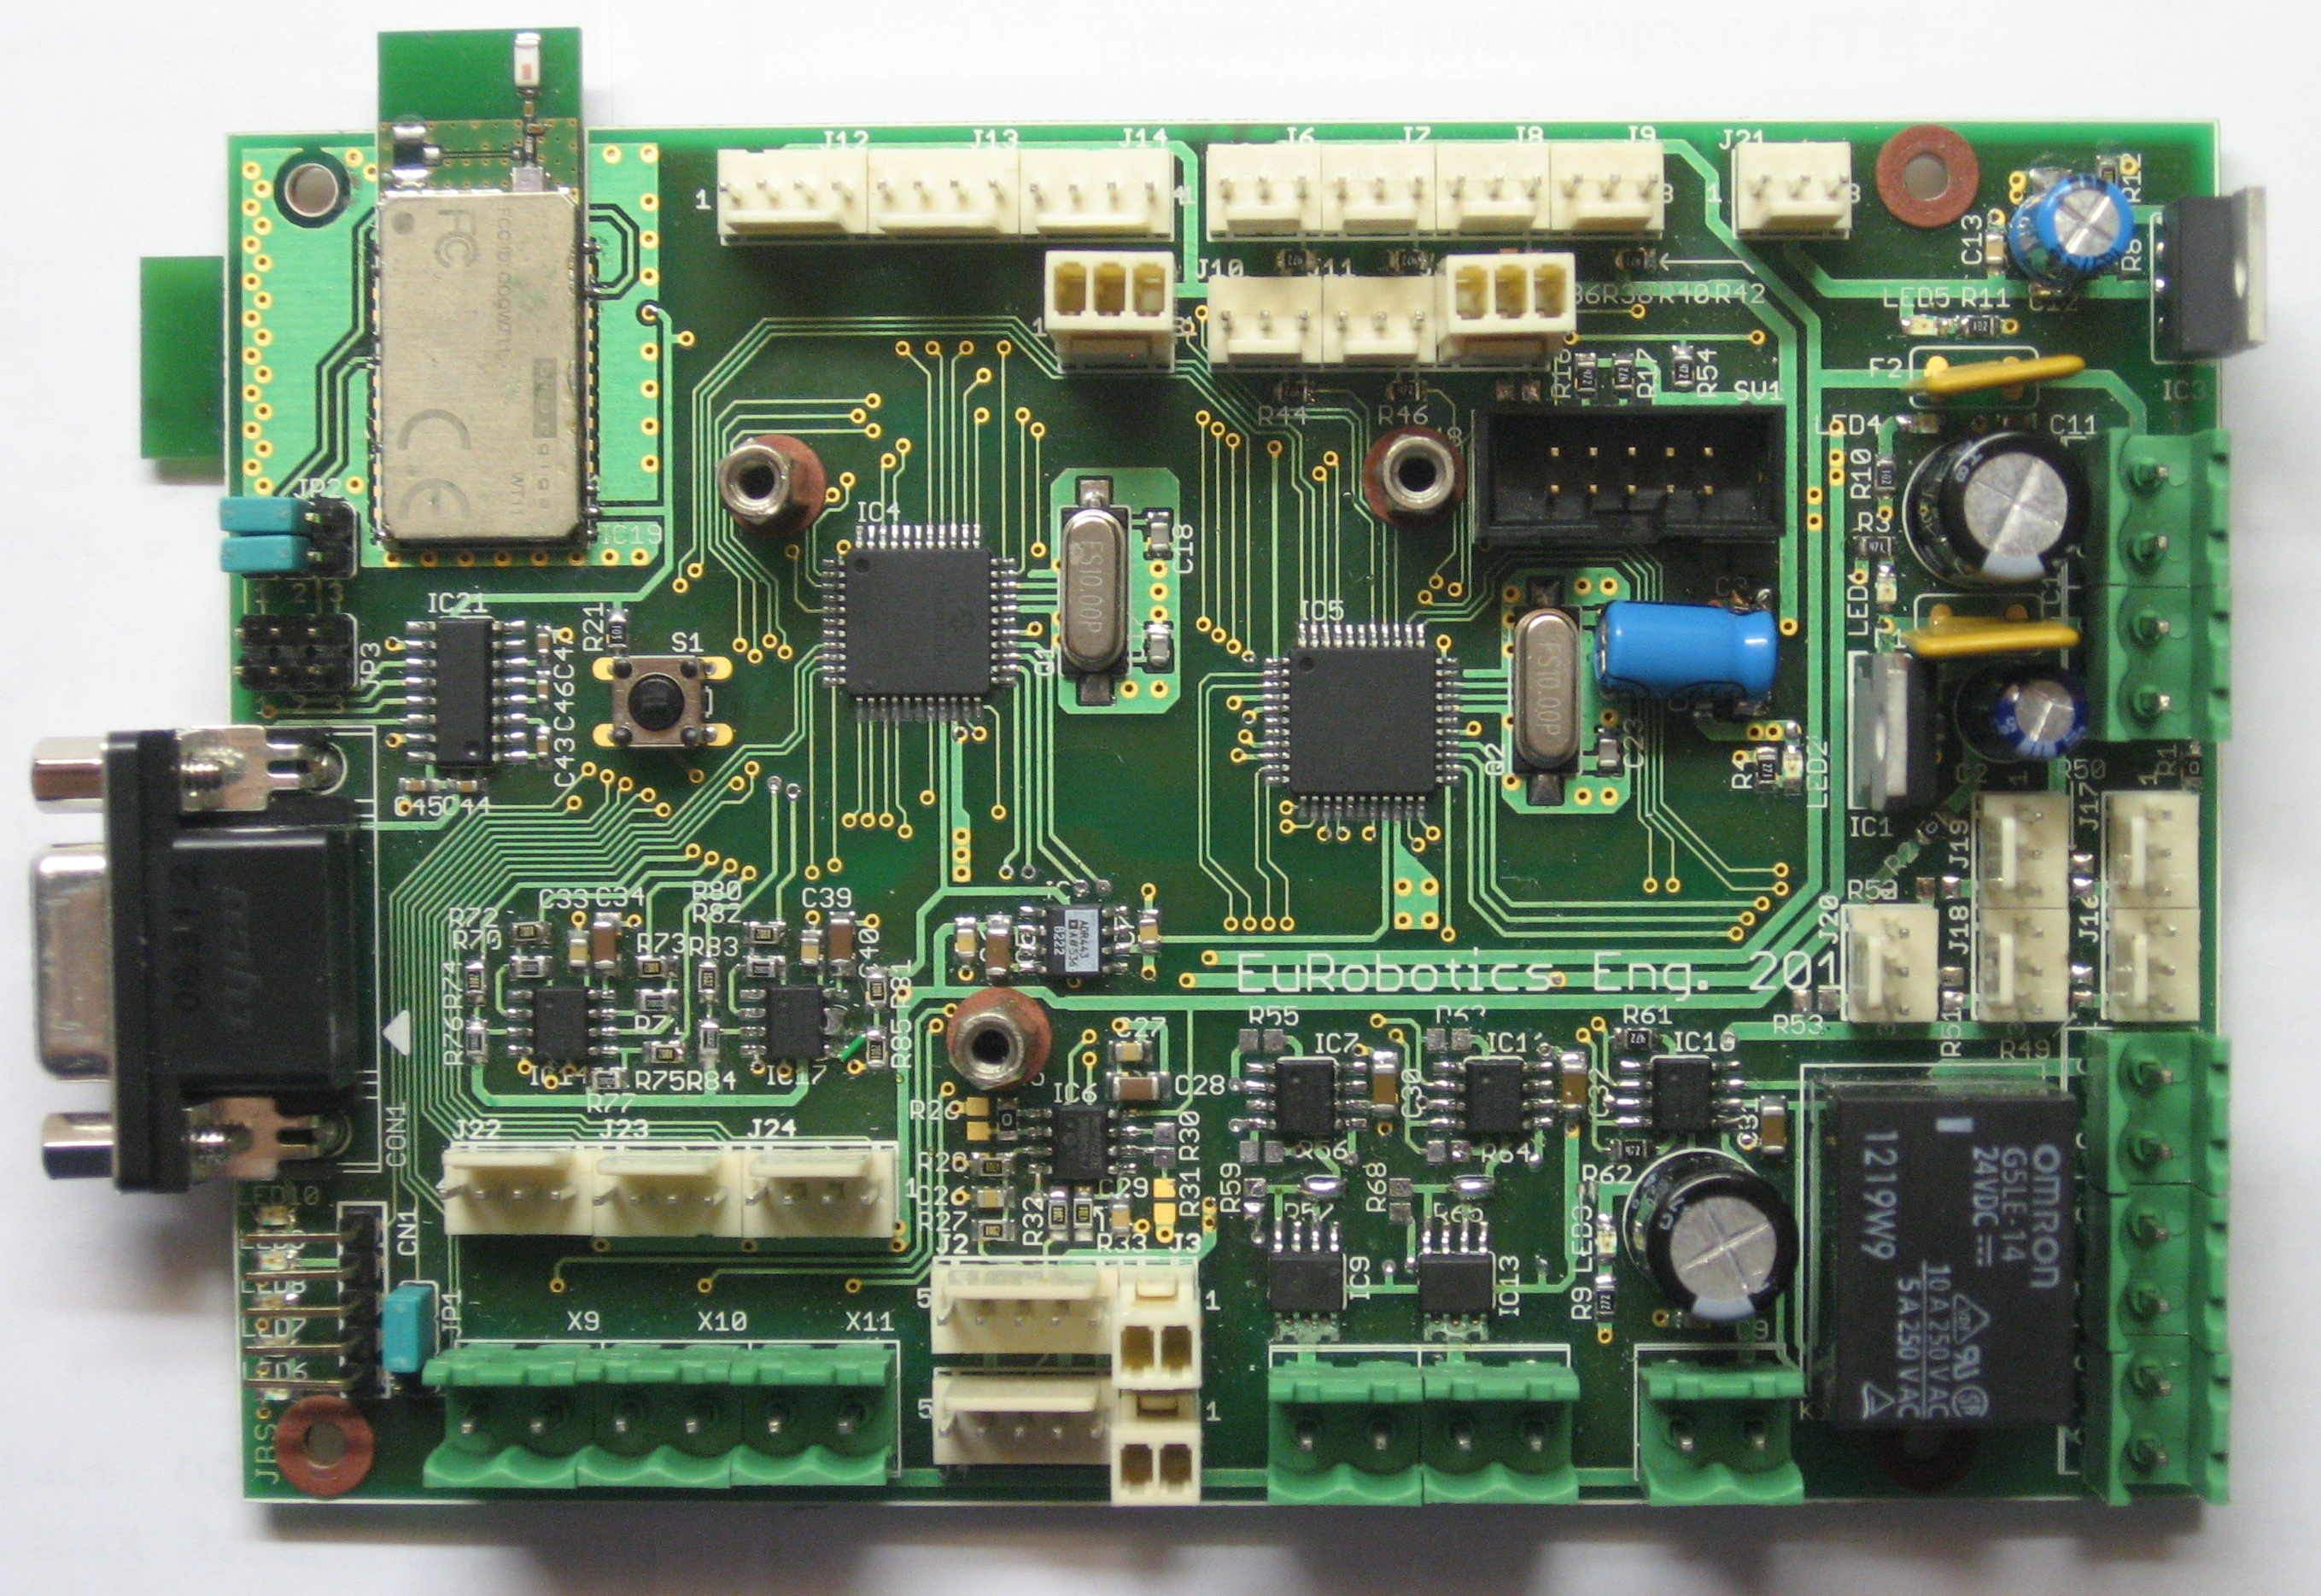
\includegraphics[width=.8\textwidth]{fotos_tarjetas/mainboard_v01_v02}
\caption[]{Tarjeta \emph{mainboard\_v02}}
\label{fig_tarjeta_mainboard_v01_v02}
\end{figure}

\subsection{Tarjeta de sensores digitales}

\begin{figure}[H]
\centering
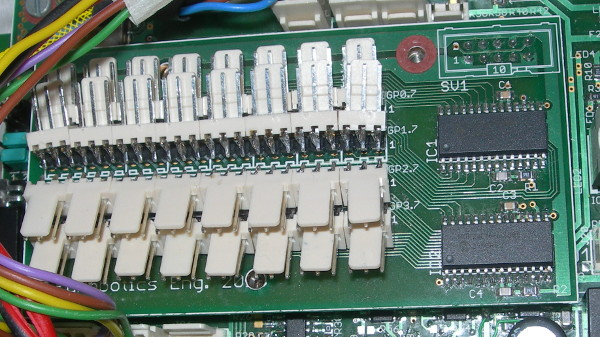
\includegraphics[width=.6\textwidth]{fotos_tarjetas/sensorboard}
\caption[]{Tarjeta \emph{sensorboard}}
\label{fig_tarjeta_sensorboard}
\end{figure}

\subsection{Tarjeta de sistemas de vacio}

\begin{figure}[H]
\centering
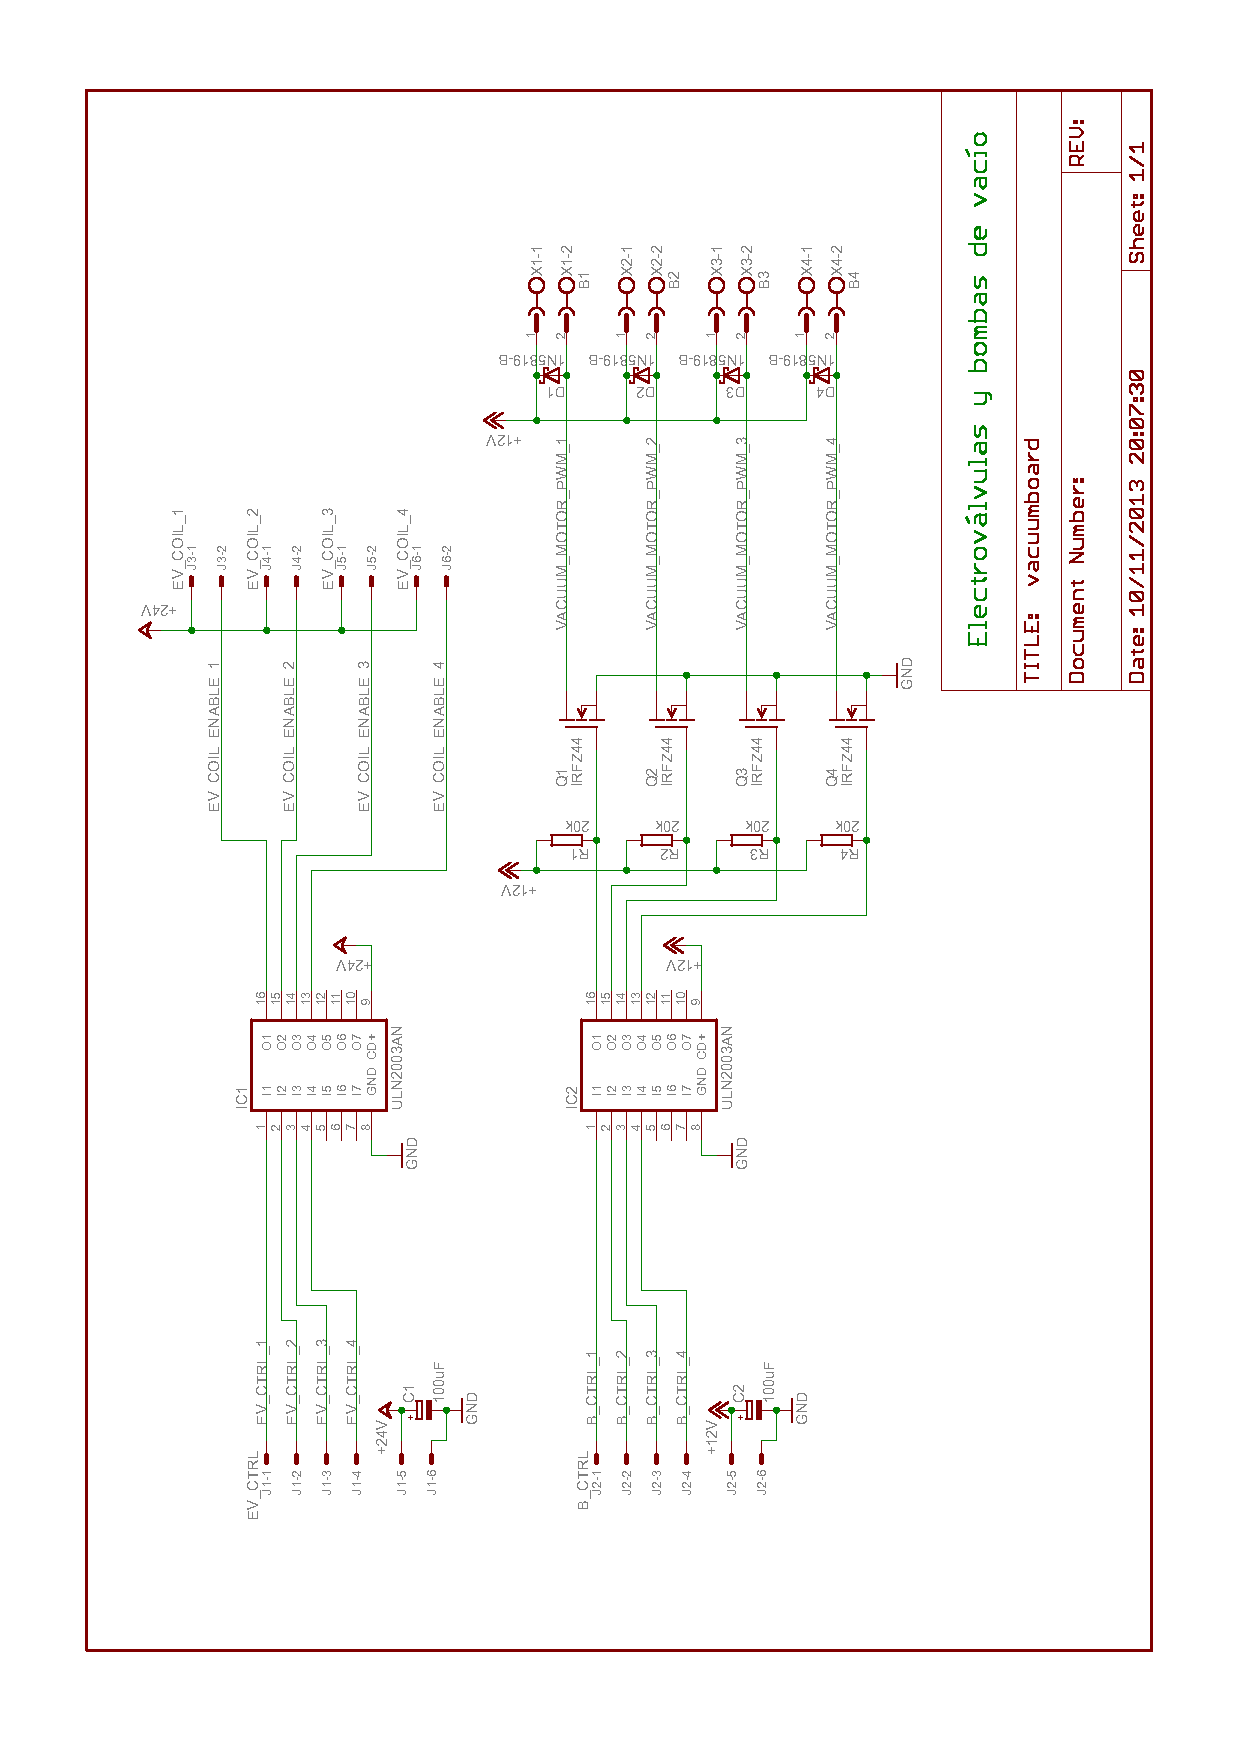
\includegraphics[width=.5\textwidth]{fotos_tarjetas/vacuumboard}
\caption[]{Tarjeta \emph{vacuumboard}}
\label{fig_tarjeta_vacuumboard}
\end{figure}

\subsection{Tarjeta de control de alimentaci�n}

\begin{figure}[H]
\centering
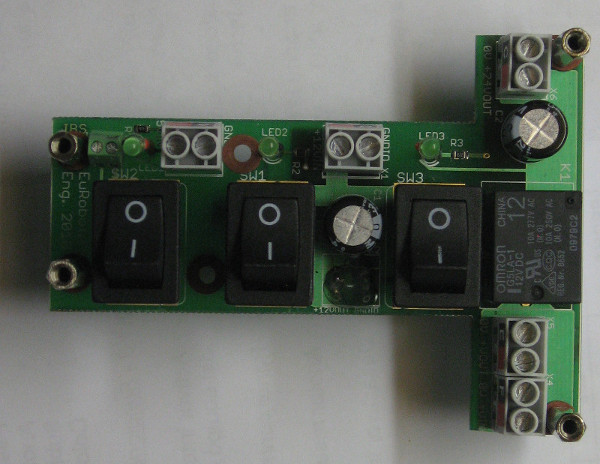
\includegraphics[width=.6\textwidth]{fotos_tarjetas/switchboard}
\caption[]{Tarjeta \emph{switchboard}}
\label{fig_tarjeta_switchboard}
\end{figure}

\subsection{Tarjeta de alimentaci�n}

\begin{figure}[H]
\centering
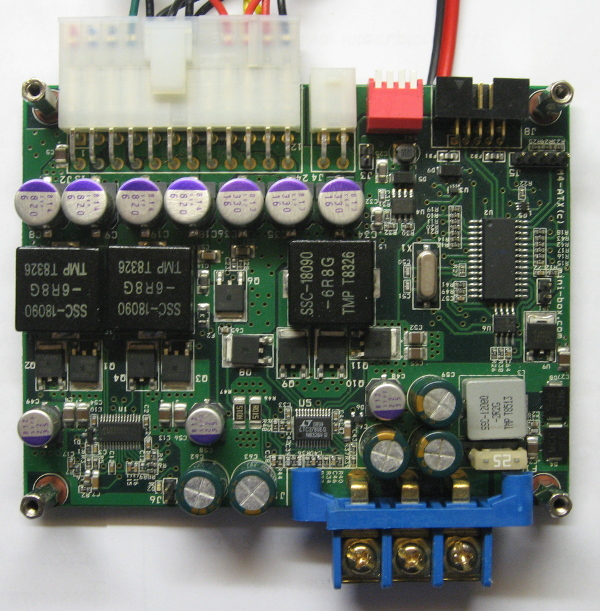
\includegraphics[width=.6\textwidth]{fotos_tarjetas/m4_atx}
\caption[]{Tarjeta \emph{M4-ATX}}
\label{fig_tarjeta_m4_atx}
\end{figure}


\section{Implementaci�n HW del robot secundario}

\begin{figure}[H]
\centering
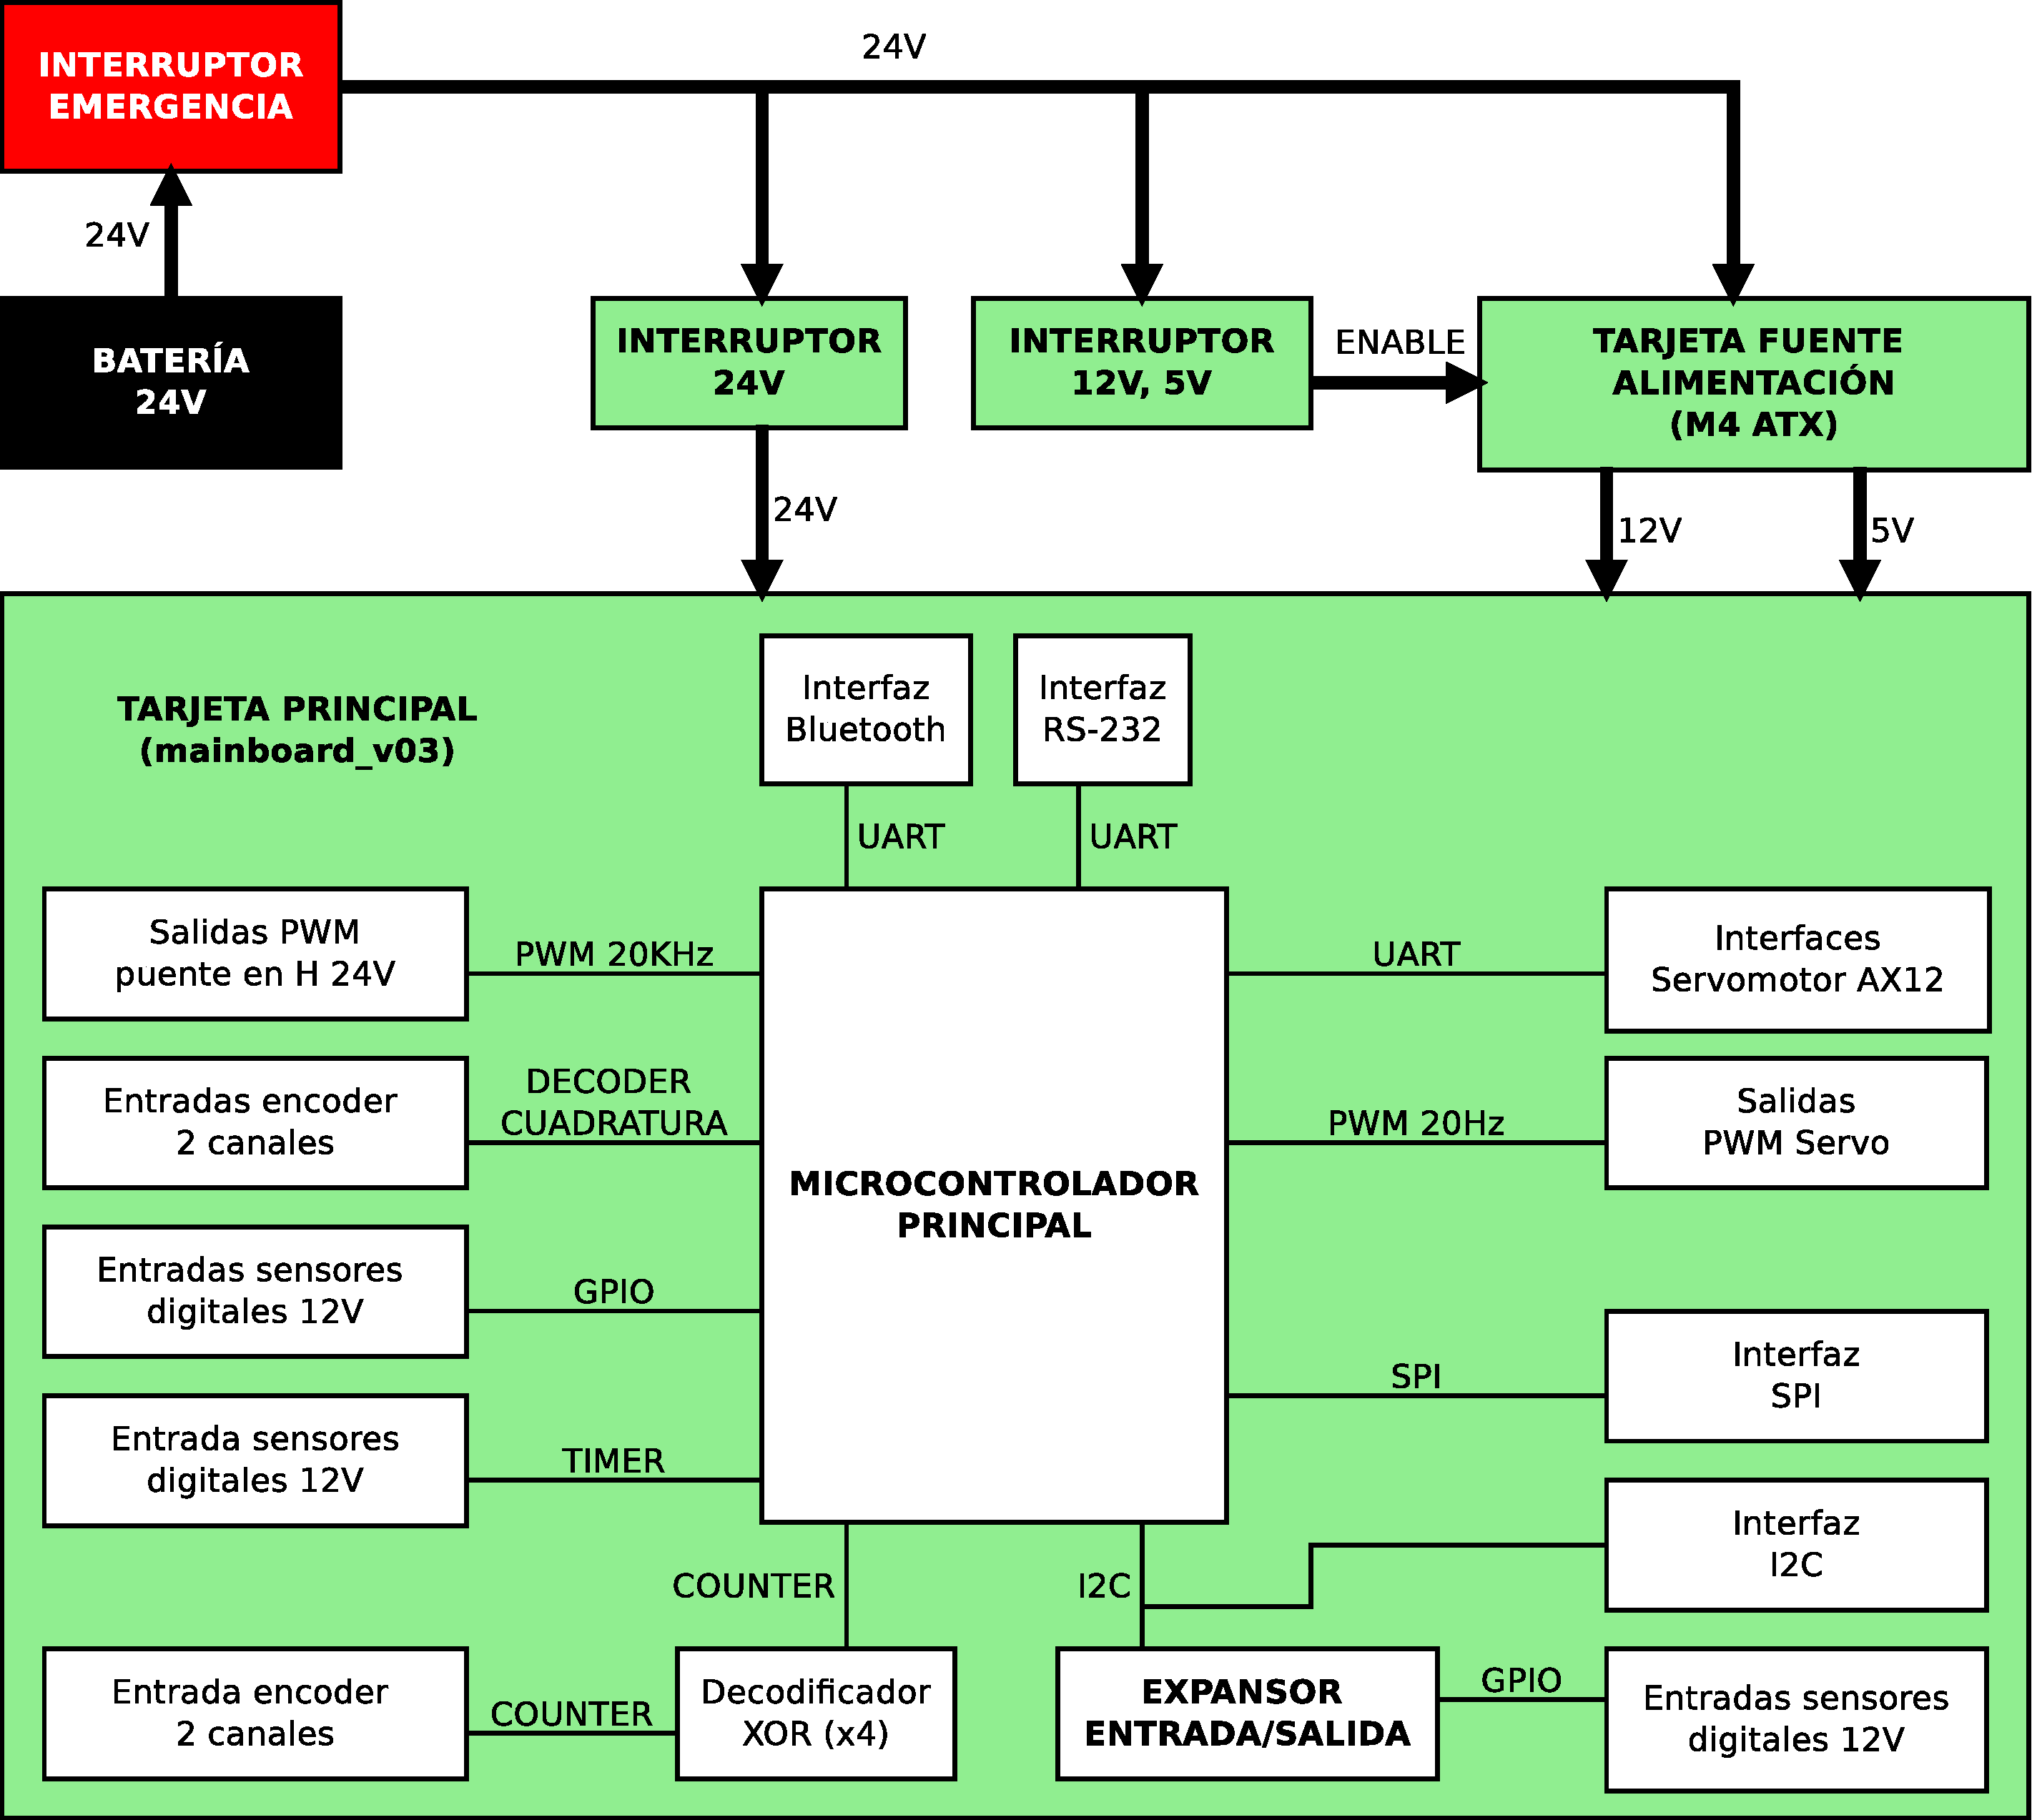
\includegraphics[width=.9\textwidth]{hardware_robot_secundario}
\caption[]{Diagrama de bloques del HW del robot secundario}
\label{fig_hardware_robot_secundario}
\end{figure}

\begin{figure}[H]
\centering
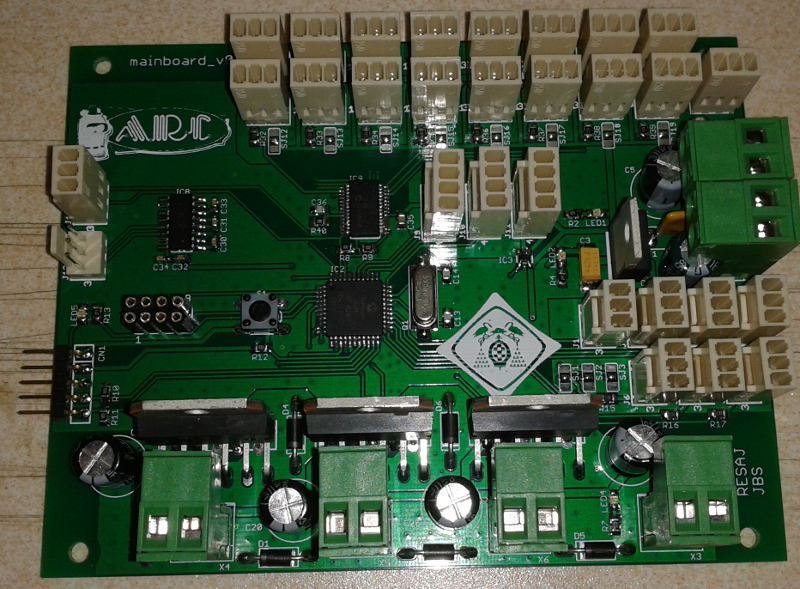
\includegraphics[width=.7\textwidth]{fotos_tarjetas/mainboard_v03}
\caption[]{Tarjeta \emph{mainboard\_v03}}
\label{fig_tarjeta_mainboard_v03}
\end{figure}


%%% Local Variables:
%%% TeX-master: "../book"
%%% End:
